\section{Evasion Attacks}

\subsection{Adversarial Patch}

Adversarial Patch, saldırganın hedef modelin karar verme sürecini manipüle etmek amacıyla görüntülerin üzerine eklediği bir "yama" (patch) kullanılarak yapılır. Bu yama, görüntüye yerleştirildiğinde modelin yanlış sınıflandırmasına neden olur. Modelin içindeki sinir ağları, görsel özellikleri inceleyerek karar verir. Adversarial Patch, bu özellikleri yanıltarak, ağırlıkların yanlış hesaplanmasını sağlar ve modelin hatalı sınıflandırma yapmasına yol açar. Saldırgan, bir optimizasyon süreci kullanarak yamayı üretir. Yamayı oluşturan piksel değerleri, modelin doğru çalışmasını bozacak şekilde optimize edilir.

\[ \min_{\delta} \mathbb{E}_{x \sim \mathcal{D}} \left[ \mathcal{L}(f(x + \delta), y_{\text{target}}) \right] \]

Burada:

\begin{itemize}
    \item $x$: Giriş görüntüsü.
    \item $\delta$: Adversarial patch.
    \item $f(x + \delta)$: Patch eklenmiş görüntü ile modelin tahmini.
    \item $y_{target}$: Hedeflenen yanlış sınıf.
    \item $\mathcal{L}$: Kayıp fonksiyonu.
\end{itemize}

\subsubsection{Çalışma Adımları}

\begin{enumerate}
    \item İlk olarak, hangi sınıflandırmanın yanlış yapılmasının istendiği belirlenir.
    \item Yamanın yerleştirileceği bölge ve büyüklük seçilir. Bu yamayı oluşturan piksel değerleri optimize edilecektir.
    \item Saldırgan, modelin tahmin hatası üzerinden yamayı optimize eder. Bunun için kullanılan optimizasyon algoritmaları yamayı, modele zarar verecek şekilde günceller.
    \item Optimizasyon tamamlandıktan sonra yamayı hedef görüntüye yerleştirir ve modelin saldırıya nasıl tepki verdiği gözlemlenir.
\end{enumerate}

\newpage

\subsection{Adversarial Texture}

Adversarial Texture, bir nesnenin yüzeyine uygulanan ve o nesnenin model tarafından yanlış tanınmasına yol açan bir "doku" ile saldırı gerçekleştirir. Adversarial Texture, temelde optimizasyon süreçleri kullanarak nesnenin görünümünü manipüle eder. Modelin tahmin performansını bozacak şekilde tasarlanmış olan bu dokular, model tarafından işlenen özellikleri yanıltarak modelin yanlış tahminler yapmasına yol açar. Bu saldırı, görüntüdeki belirli bir dokuya odaklanarak yapıldığı için daha geniş ve nesnenin genel yapısını etkileyen bir saldırı olarak kabul edilir.

\[ \min_{T} \mathbb{E}_{x \sim \mathcal{D}} \left[ \mathcal{L}(f(T(x)), y_{\text{target}}) \right] \]

Burada:

\begin{itemize}
    \item $x$: Giriş görüntüsü.
    \item $T(x)$: Manipüle edilmiş dokuya sahip görüntü.
    \item $f(T(x))$: Modelin dokulu görüntüyle verdiği tahmin.
    \item $y_{target}$: Hedeflenen yanlış sınıf.
    \item $\mathcal{L}$: Kayıp fonksiyonu.
\end{itemize}

\subsubsection{Çalışma Adımları}

\begin{enumerate}
    \item İlk olarak, hangi modelin ve hangi nesnenin hedefleneceği belirlenir.
    \item Saldırgan, modelin tahmin performansını bozacak şekilde dokuyu tasarlar.
    \item Doku, modelin sınıflandırma doğruluğunu bozacak şekilde optimize edilir. Bu süreçte kayıp fonksiyonu minimize edilir ve doku, hedeflenen yanlış sınıfı oluşturacak şekilde güncellenir.
    \item Optimizasyon sonucunda elde edilen doku, nesneye uygulanır ve modelin saldırıya nasıl tepki verdiği gözlemlenir.
\end{enumerate}

\newpage

\subsection{Auto Projected Gradient Descent (Auto-PGD)}

Auto-PGD, bir modelin saldırılara karşı dayanıklılığını (adversarial robustness) test etmek için kullanılan bir saldırı yöntemidir. Auto-PGD, PGD'nin iyileştirilmiş bir versiyonudur ve modelin güvenliğini daha etkin bir şekilde test etmek için otomatik olarak optimizasyon parametrelerini belirler. 

Auto-PGD'nin temel mantığı, modelin kayıp fonksiyonunun gradyanını hesaplayarak adversarial örnekler üretmektir. Bu süreç birkaç iterasyon boyunca devam eder ve üretilen adversarial örnekler, modelin kararlılığına zarar vererek modelin yanlış sınıflandırmalar yapmasını sağlar. Auto-PGD, belirlenen bir sınır içinde kalarak en etkin saldırıyı bulmaya çalışır.

\[ x^{t+1} = \text{Proj}_{\mathcal{B}(x, \epsilon)} \left( x^t + \alpha \cdot \frac{\nabla_x \mathcal{L}(f(x^t), y)}{\|\nabla_x \mathcal{L}(f(x^t), y)\|_p} \right) \]

Burada:

\begin{itemize}
    \item $x^t$: t-inci adımda üretilen adversarial örnek.
    \item $\alpha$: İterasyon başına yapılan adım büyüklüğü.
    \item $\mathcal{L}(f(x^t), y)\|$ Modelin kayıp fonksiyonunun giriş verisine göre gradyanı.
    \item $\text{Proj}_{\mathcal{B}(x, \epsilon)}$: Girişin $\epsilon$-norm sınırları içinde kalmasını sağlayan projeksiyon.
    \item $p$: Norm tipi (genellikle $L_\infty$ normu kullanılır.)
\end{itemize}

\subsubsection{Çalışma Adımları}

\begin{enumerate}
    \item İlk olarak saldırılacak model ve veri seti seçilir.
    \item Pertürbasyon için belirli bir sınır tanımlanır. Bu sınır, saldırının şiddetini belirler.
    \item Modelin kayıp fonksiyonunun giriş verisine göre gradyanı hesaplanır. Bu gradyan, hangi yönde saldırı yapılacağını gösterir.
    \item Hesaplanan gradyanlar kullanılarak giriş verisi üzerinde değişiklikler yapılır, ancak yapılan bu değişiklikler belirlenen $\epsilon$-norm sınırları içinde kalacak şekilde projeksiyon uygulanır.
    \item Bu süreç birkaç iterasyon boyunca tekrarlanır.
\end{enumerate}

\newpage

\subsection{Auto Conjugate Gradient (Auto-CG)}

Auto-CG, Conjugate Gradient (CG) optimizasyon yöntemine dayanır. Auto-CG, modelin kayıp fonksiyonunu minimize etmek için conjugate gradient yaklaşımını kullanır ve bu optimizasyon yöntemi ile adversarial örnekler üretir. Auto-CG, conjugate gradient algoritmasının otomatikleştirilmiş ve model güvenliği için optimize edilmiş bir versiyonudur. Conjugate Gradient (CG) yöntemi, gradyan tabanlı optimizasyon yöntemlerinin geliştirilmiş bir şeklidir. Bu yöntem, özellikle büyük boyutlu problem setlerinde daha hızlı ve daha etkin bir optimizasyon sağlar. CG algoritması, modelin kayıp fonksiyonunun gradyanını hesaplar ve conjugate (eşlenik) yönünde adım atarak hedef fonksiyonu minimize etmeye çalışır.

Auto-CG'nin temel formülü, conjugate gradient algoritmasındaki adım güncellemesini kullanır. İteratif olarak, her adımda giriş verisi $x$, conjugate direction (eşlenik yön) boyunca güncellenir.

\[ x^{t+1} = x^t + \alpha^t d^t \]

Burada:

\begin{itemize}
    \item $x^t$: t-inci iterasyondaki veri örneği.
    \item $\alpha^t$: İterasyon başına adım büyüklüğü.
    \item $d^t$: Conjugate (eşlenik) yön.
\end{itemize}

\subsubsection{Çalışma Adımları}

\begin{enumerate}
    \item Model ve veri seti seçilir.
    \item Saldırı için bir başlangıç örneği seçilir ve bu örnek üzerinde iterasyonlar yapılır.
    \item Modelin kayıp fonksiyonu, giriş veri üzerinde gradyanı hesaplayarak optimize edilir.
    \item Conjugate Gradient yöntemine uygun olarak eşlenik yön hesaplanır ve bu yön boyunca adım atılır.
    \item Her adımda daha etkili bir adversarial örnek üretilir.
    \item Yapılan değişikliklerin belirli bir $\epsilon$-norm içinde kalması için projeksiyon adımı uygulanır.
\end{enumerate}

\newpage

\subsection{Boundary Attack (Decision-Based Attack)}

Boundary Attack, karara dayalı bir saldırı yöntemidir. Bu saldırı, modelin iç yapısını veya gradyan bilgilerini kullanmadan, yalnızca modelin verdiği kararlar (etiketler) üzerinden çalışır. Boundary Attack, modelin yanlış sınıflandırmasını sağlamak için, verinin sınırına (decision boundary) en yakın olan yanlış sınıflandırılan örneği bulmaya çalışır. Bu yöntem, örneği kademeli olarak modelin karar sınırına iterek çalışır.

Boundary Attack, rastgele bir örnekten başlar ve bu örneğe küçük pertürbasyonlar ekleyerek, modelin karar sınırına en yakın yanlış sınıflandırılan örneği bulmaya çalışır. Bu yöntemle, modelin verdiği kararları gözlemleyerek (etiketlere dayanarak) örneği değiştirmeyi amaçlar.

\subsubsection{Çalışma Adımları}

\begin{enumerate}
    \item Saldırı, rastgele bir örnekten başlar. Bu, modelin karar sınırına uzak bir örnektir.
    \item Rastgele seçilen bu örneğin karar sınırına doğru ilerletilmesi gerekir. Bunun için, modelin sınıflandırma kararlarını kullanarak, veri noktasına küçük değişiklikler yapılır.
    \item Adversarial örnek, modelin yanlış sınıflandırılması gereken karar sınırına mümkün olduğunca yakın hale getirilmeye çalışılırken, aynı zamanda minimum düzeyde pertürbasyon eklenir.
    \item Her iterasyonda, pertürbasyon küçülür ve sınırdaki en küçük değişimlerle hedeflenen sınıflandırmaya ulaşılmaya çalışılır.
\end{enumerate}

\newpage

\subsection{Brendel and Bethge (B\&B) Attack}

B\&B Attack, karar tabanlı bir saldırı yöntemidir. Bu saldırı, modelin karar sınırına en yakın yanlış sınıflandırılan bir örnek bulmayı hedefler. Black-box bir saldırı türü olduğundan, saldırgan modelin gradyanlarına, iç yapısına veya ağırlıklarına erişime ihtiyaç duymaz, yalnızca modelin verdiği kararları (etiketleri) kullanır. Bu saldırı, özellikle modelin yanlış sınıflandırmasına yol açacak minimum pertürbasyonları üretmek amacıyla, modelin verdiği kararları optimize ederek çalışır. Boundary Attack ile benzerlik gösterse de, Brendel and Bethge Attack daha hassas ve ince ayarlı bir saldırı mekanizması kullanır.

Brendel and Bethge Attack, modelin kararlarına göre giriş verisine minimal değişiklikler yapar. Pertürbasyon $\delta$, giriş verisine $x$ şu şekilde uygulanır:

\[ x_{\text{adv}} = x + \delta \]

\subsubsection{Çalışma Adımları}

\begin{enumerate}
    \item İlk adımda, yanlış sınıflandırılan bir örnek seçilir.
    \item Modelin karar sınırına en yakın olan noktayı bulmak için küçük ve optimize edilmiş pertürbasyonlar eklenir. Bu adımda, modelin kararlarını gözlemleyerek minimum düzeyde değişiklikler yapılır.
    \item Pertürbasyonlar modelin verdiği kararlarla kıyaslanır ve her iterasyonda sınırdaki yanlış sınıflandırmayı bulmak hedeflenir.
    \item Her iterasyonda pertürbasyonlar optimize edilir, böylece yanlış sınıflandırılan en yakın sınırdaki örnek bulunmaya çalışılır.
\end{enumerate}

\newpage

\subsection{Carlini and Wagner L0 Attack}

C\&W L0 Attack, Carlini and Wagner tarafından geliştirilmiştir. Amacı, modellerin yanlış sınıflandırma yapmasına neden olmak için en az sayıda pikseli değiştirmektir. L0 normunu minimize eden bu saldırı, pertürbasyonların en az sayıda pikselde yapılmasını sağlar.

L0 normu, bir vektörde sıfır olmayan elemanların sayısını ifade eder. C\&W L0 saldırısı, görüntüdeki minimum sayıda pikseli değiştirerek modeli yanlış sınıflandırmaya zorlar. Bu, saldırının insan gözünde çok zor fark edilebilecek kadar küçük değişikliklerle yapılmasını sağlar.

\[ \min \|x' - x\|_0 \quad \text{subject to} \quad f(x') = t \]

Burada:

\begin{itemize}
    \item $x$: Giriş görüntüsü.
    \item $x'$: Adversarial örnek.
    \item $t$: Hedef sınıf.
    \item $\min \|x' - x\|_0$: L0 normu, değiştirilen piksel sayısı.
\end{itemize}

\subsubsection{Çalışma Adımları}

\begin{enumerate}
    \item İlk olarak, doğru sınıflandırılan bir görüntü alınır.
    \item Amaç ya bir hedef sınıfa yönelik saldırı gerçekleştirmek (targeted attack) ya da yanlış bir sınıflandırma yaratmaktır (non-targeted attack).
    \item Saldırı, giriş görüntüsüne eklenmesi gereken en küçük değişiklikliği bulmak için bir optimizasyon problemi çözer. Bu adımda, mümkün olan en az sayıda piksel değiştirilir ve bozulma sınırlanır.
    \item Yapılan değişiklikler, modelin yanlış sınıflandırmasını sağlayana kadar optimize edilir. Bu işlem sırasında saldırı, L0 normunu minimize eder.
\end{enumerate}

\newpage

\subsection{Carlini and Wagner L2 Attack}

C\&W L2 saldırısı, giriş görüntüsüne eklenen bozulmayı L2 normuna göre optimize ederek, modelin yanlış sınıflandırma yapmasına neden olur. L2 normu, giriş görüntüsüne en az bozulmayı ekleyerek modeli yanıltmayı amaçlar. Amaç, modelin sınıflandırmasını bozmak için görüntüye çok küçük ama stratejik değişiklikler yapmaktır. C\&W L2 saldırısı, bozulmaların toplam büyüklüğünü minimize eder ve bu sayede insan gözünün algılaması zor olan adversarial örnekler oluşturur.

\[ \min \|x' - x\|_2^2 + c \cdot f(x') \]

Burada:

\begin{itemize}
    \item $x$: Giriş görüntüsü.
    \item $x'$: Adversarial örnek.
    \item $\min \|x' - x\|_2$: L2 normu, yani giriş görüntüsü ile adversarial örnek arasındaki farkın büyüklüğü.
    \item $f(x')$: Modelin sınıflandırma kaybı.
    \item $c$: Kayıp fonksiyonunu dengeleyen bir sabit.
\end{itemize}

\newpage

\subsection{Carlini and Wagner L$\infty$ Attack}

C\&W L$\infty$, belirli bir giriş görüntüsüne maksimum bir bozulma ekleyerek modelin yanlış sınıflandırmasını sağlamayı amaçlar. L$\infty$ normu, bir görüntüdeki en büyük piksek değişikliğini sınırlayarak adversarial örnekler oluşturur. 

\[ \min \|x' - x\|_\infty + c \cdot f(x') \]

Burada:

\begin{itemize}
    \item $x$: Giriş görüntüsü.
    \item $x'$: Adversarial örnek.
    \item $\min \|x' - x\|_2$: L2 normu, yani giriş görüntüsü ile adversarial örnek arasındaki farkın büyüklüğü.
    \item $f(x')$: Modelin sınıflandırma kaybı.
    \item $c$: Kayıp fonksiyonunu dengeleyen bir sabit.
\end{itemize}

\newpage

\subsection{Carlini and Wagner ASR Attack}

Otmatik konuşma sistemlerini hedef alır. Bu saldırı, konuşma tanıma sistemlerinin verdiği çıktıları manipüle etmek için adversarial ses sinyalleri üretir. Amacı, insanların algılayamayacağı seviyede ses bozulmaları oluşturarak bir ses kaydını, ASR sistemlerinde yanlış şekilde tanınan veya hedeflenen bir komut haline getirmektir.

\[ \min \|x' - x\|_2 + c \cdot f(x') \]

Burada:

\begin{itemize}
    \item $x$: Giriş sinyali.
    \item $x'$: Adversarial örnek.
    \item $\min \|x' - x\|_2$: L2 normu, yani giriş sinyali ile adversarial örnek arasındaki farkın büyüklüğü.
    \item $f(x')$: Modelin sınıflandırma kaybı.
    \item $c$: Kayıp fonksiyonunu dengeleyen bir sabit.
\end{itemize}

\subsubsection{Çalışma Adımları}

\begin{enumerate}
    \item Hedef model ve sinyal seçilir.
    \item Saldırı hedefinin yanlış tanımlanmış bir komut ya da belirli bir hedef komut olması beklenir.
    \item ASR sistemini yanlış sonuç vermeye yönlendirecek en küçük pertürbasyonlar hesaplanır.
    \item Bu bozulmalar, L2 normu veya başka bir noma göre optimize edilerek saldırı güçlendirilir.
\end{enumerate}

\newpage

\subsection{Composite Adversarial Attack}

Composite Adversarial Attack, farklı türdeki evasion saldırılarını bir araya getirerek çoklu saldırı stratejileridir. Birkaç farklı saldırı yöntemi ardışık olarak uygulanır ya da bir araya getirilir. Amacı, bir modelin sadece tek bir saldırıya karşı değil, birden fazla saldırıya karşı dayanıklılığını test etmektir. 

\[ x' = S_2(S_1(x)) \]

Burada:

\begin{itemize}
    \item $x$: Orijinal girdi.
    \item $S_1(x)$: İlk saldırı tarafından modifiye edilen girdidir.
    \item $S_2(x')$: İkinci saldırı tarafından modifiye edilen girdidir.
\end{itemize}

\subsubsection{Python Kodu}

\begin{lstlisting}[language=Python]
from art.estimators.classification import TensorFlowV2Classifier
from art.attacks.evasion import FastGradientMethod, ProjectedGradientDescent

art_model = TensorFlowV2Classifier(
    model=model, 
    loss_object=SparseCategoricalCrossentropy(from_logits=True), 
    nb_classes=10, input_shape=(784,), clip_values=(0, 1))

pgd = ProjectedGradientDescent(estimator=art_model, targeted=False, 
                               eps=0.1, eps_step=0.01, max_iter=40)

x_test_adv_fgsm = fgsm.generate(x_test)
x_test_adv_composite = pgd.generate(x=x_test_adv_fgsm)
\end{lstlisting}

\newpage

\begin{figure}[h]
    \centering
    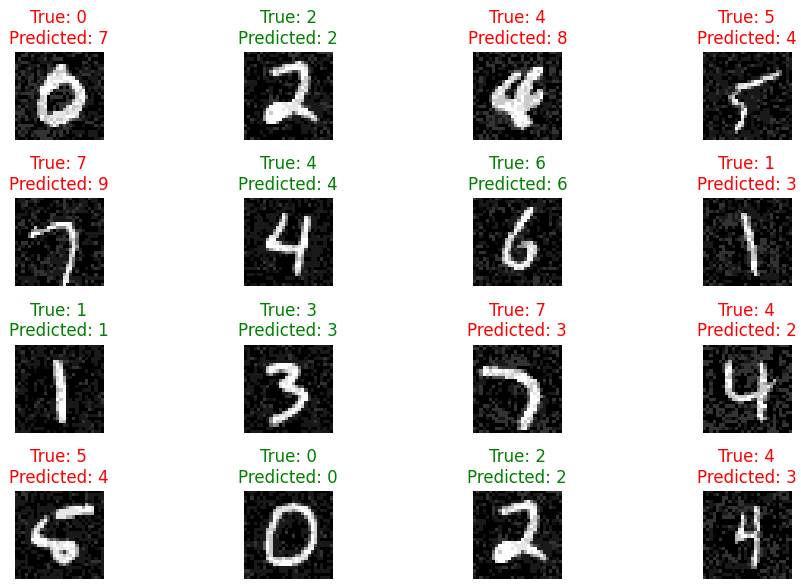
\includegraphics[width=1\textwidth]{images/composite_adversarial_attack_results.png}
    \caption{}
\end{figure}

\newpage

\subsection{Decision Tree Attack}

Decision Tree Attack, karar ağacının düğümlerini ve dallarını hedef alarak saldırı oluşturur. Bu saldırı türünde, giriş verileri yavaş yavaş değiştirerek, birden fazla düğümde farklı kararlar alınmasını sağlar. Böylelikle, modelin çıktısını yanlış bir yöne yönlendirmek için küçük ama etkili değişiklikler yapılır.

\subsubsection{Çalışma Adımları}

\begin{enumerate}
    \item İlk olarak, modelin karar ağacı yapısı analiz edilir ve modelin nasıl çalıştığı anlaşılır.
    \item Karar ağacının her bir dalı boyunca, giriş verilerinde küçük değişiklikler yaparak saldırgan örnekler oluşturulur.
    \item Giriş verileri optimize edilerek modelin verdiği kararı yanlış yöne kaydıracak en iyi adversarial örnek bulunur.
    \item Karar ağacındaki zayıf noktalar tespit edildikten sonra, model bu zayıflıkları kullanarak saldırıya uğratılır.
\end{enumerate}

\subsubsection{Python Kodu}

\begin{lstlisting}[language=Python]
from art.estimators.classification import SklearnClassifier
from art.attacks.evasion import DecisionTreeAttack
art_dt = SklearnClassifier(model=dt)
attack = DecisionTreeAttack(art_dt)
adv_test = attack.generate(x_test)
\end{lstlisting}

\begin{figure}[h]
    \centering
    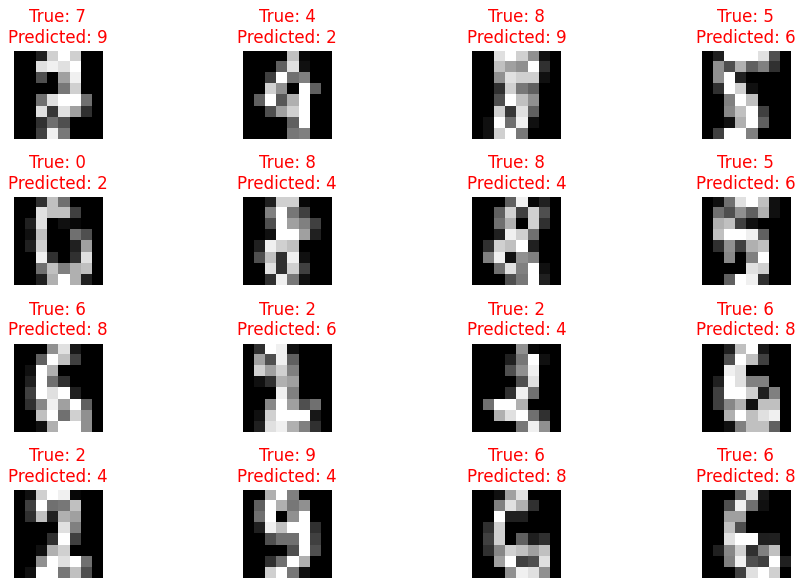
\includegraphics[width=0.6\textwidth]{images/dt_attack_results.png}
    \caption{}
\end{figure}

\newpage

\subsection{Deep Fool}

DeepFool, giriş verilerini sınırlı miktarda değiştirerek (pertürbe ederek), bu verilerin sınıflandırılmasını değiştirmeye çalışır. Amaç, orijinal sınıf ile yanlış sınıf arasında minimum değişikliklerle adversarial bir örnek oluşturmaktır. DeepFool, temelde karar sınırlarına en yakın olan minimum pertürbasyonu bulur ve bu pertürbasyonla sınıflandırmayı değiştirir.

\[ r = \frac{| f(x) |}{\|\nabla f(x)\|} \]

Burada:

\begin{itemize}
    \item $x$: Giriş verisi.
    \item $f(x)$: Modelin karar fonksiyonu.
    \item $\nabla f(x)$: Karar fonksiyonunun gradyanı.
    \item $r$: Giriş verisine eklenen pertürbasyon.
\end{itemize}

\subsubsection{Çalışma Adımları}

\begin{enumerate}
    \item İlk olarak modelin doğru sınıflandırdığı bir giriş verisi alınır.
    \item Modelin karar sınırları tespit edilir ve sınıf değiştirmek için gerekli minimum pertürbasyon hesaplanır.
    \item Hesaplanan küçük bir pertürbasyon giriş verisine eklenir.
    \item Bu işlem tekrarlanarak modelin sınıflandırmasını değiştirecek minimum pertürbasyon elde edilir.
\end{enumerate}

\subsubsection{Python Kodu}

\begin{lstlisting}[language=Python]
from art.estimators.classification import TensorFlowV2Classifier
from art.attacks.evasion import DeepFool

art_model = TensorFlowV2Classifier(
    model=model, 
    loss_object=SparseCategoricalCrossentropy(from_logits=True), 
    nb_classes=10, input_shape=(784,), clip_values=(0, 1))

deep_fool = DeepFool(classifier=art_model)
adv_test = deep_fool.generate(x=x_test)
\end{lstlisting}

\newpage

\begin{figure}[h]
    \centering
    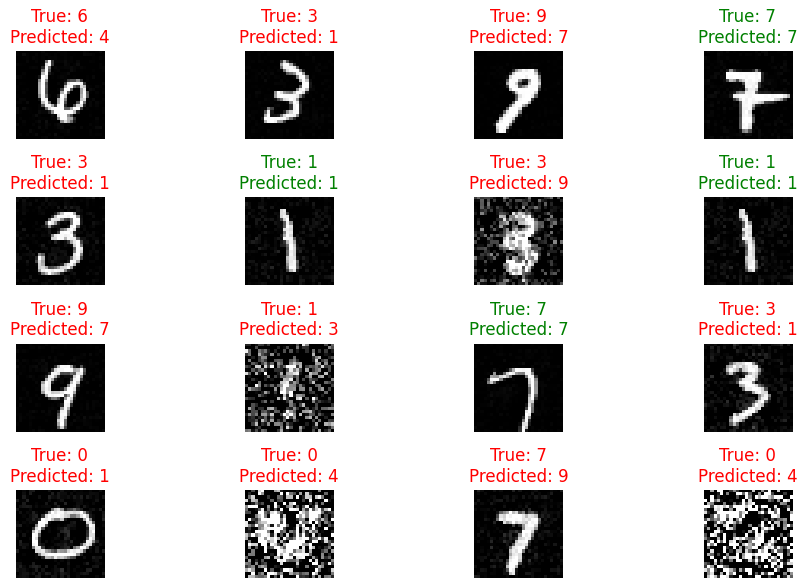
\includegraphics[width=1\textwidth]{images/deep_fool_attack_results.png}
    \caption{}
\end{figure}

\newpage

\subsection{DPatch}

DPatch Attack, sahnede belirli bir konuma küçük bir pertürbasyon yerleştirir ve bu sayede görüntüdeki diğer nesneler veya özellikler ne kadar net olursa olsun modelin çıktısını manipüle edebilir. Bu patch, modelin karar verme sürecini etkiler ve doğru sınıflandırmayı engeller. Bu saldırı, modelin girişindeki patch'e odaklanmasını sağlar ve bu sayede diğer özellikler göz ardı edilir.

\newpage

\subsection{Robust DPatch}

Robust DPatch Attack, DPatch'in daha gelişmiş ve dayanıklı bir versiyonudur. Robust DPatch Attack, görüntü üzerinde belirli bir bölgeye (patch) küçük ama etkili bir pertürbasyon ekler ve bu patch, modelin tahminlerini saptırmak için optimize edilir. Bu patch, modelin dikkati başka yerlerde olsa dahi sınıflandırma kararını etkiler. Bu saldırı, modelin kararlarını manipüle etmek için optimizasyon sürecini kullanır ve "patch" boyutunu küçük tutarak saldırının fark edilmemesini sağlar.

\[ \min_\delta L(f(x + \delta), y_{\text{target}}) \]

Burada:

\begin{itemize}
    \item $L$: Kayıp fonksiyonu.
    \item $f$: Modelin tahmin fonksiyonu.
    \item $x$: Orijinal görüntü.
    \item $\delta$: Patch tarafından eklenen pertürbasyon.
    \item $y_{target}$: Hedeflenen yanlış sınıf.
\end{itemize}

\newpage

\subsection{ElasticNet Attack}

ElasticNet Attack, hem $L_1$ hem de $L_2$ normlarını kullanarak saldırı yapılacak pertürbasyonun seyrekliğini ve büyüklüğünü kontrol eder. Carlini and Wagner'in bir uzantısı olarak görülen bu saldırı, çok sayıda sıfır değerli (sparse) bileşen içeren pertürbasyonlar oluşturmayı amaçlar. $L_1$-norm seyrekliği, $L_2$-norm ise pertürbasyonun büyüklüğünü kontrol eder.
\[ \min_\delta \lambda \|\delta\|_1 + (1 - \lambda) \|\delta\|_2^2 + c \cdot f(x + \delta) \]

Burada:

\begin{itemize}
    \item $\delta$: Pertürbasyon.
    \item $\|\delta\|_1$: Pertürbasyonun $L_1$-normu (seyreklik ölçütü).
    \item $\|\delta\|_2^2$: Pertürbasyonun $L_2$-normu (pertürbasyonun büyüklük ölçütü).
    \item $f(x + \delta)$: Modelin tahmin fonksiyonu.
    \item $\lambda$: $L_1$ ve $L_2$ normları arasında dengeyi sağlayan katsayı.
    \item $c$: Sınıflandırma hatasını cezalandıran sabit.
\end{itemize}

\newpage

\subsection{Fast Gradient Method (FGM)}

FGM, modelin gradyanlarını kullanarak giriş verisine ufak bir pertürbasyon ekler. Eklenen bu pertürbasyon, modein tahminini yanlış sınıfa kaydırmaya çalışır. Fast Gradient Sign Method (FGSM) ise bu saldırının bir varyasyonudur ve pertürbasyonu sadece girdinin işareti yönünde ekleyerek gerçekleştirilir. Saldırının büyüklüğünü kontrol etmek için $\epsilon$ parametresi kullanılır. $\epsilon$, pertürbasyonun ne kadar büyük olacağını belirler.

\[ x_{adv} = x + \epsilon \cdot \text{sign}(\nabla_x J(\theta, x, y)) \]

Burada:

\begin{itemize}
    \item $x_{adv}$: Adversarial girdi.
    \item $x$: Orijinal girdi.
    \item $\epsilon$: Pertürbasyon büyüklüğünü belirleyen bir parametre.
    \item $\nabla_x J(\theta, x, y)$: Modelin kayıp fonksiyonunun girdi üzerindeki gradyanı.
    \item $\text{sign}$: Gradyanın işaretini belirten fonksiyon.
\end{itemize}

\subsubsection{Python Kodu}

\begin{lstlisting}[language=Python]
from art.estimators.classification import TensorFlowV2Classifier
from art.attacks.evasion import FastGradientMethod

art_model = TensorFlowV2Classifier(
    model=model, 
    loss_object=SparseCategoricalCrossentropy(from_logits=True), 
    nb_classes=10, input_shape=(784,), clip_values=(0, 1))

fgsm = FastGradientMethod(estimator=art_model, eps=0.1)
adv_test = fgsm.generate(x=x_test)
\end{lstlisting}

\newpage

\begin{figure}[h]
    \centering
    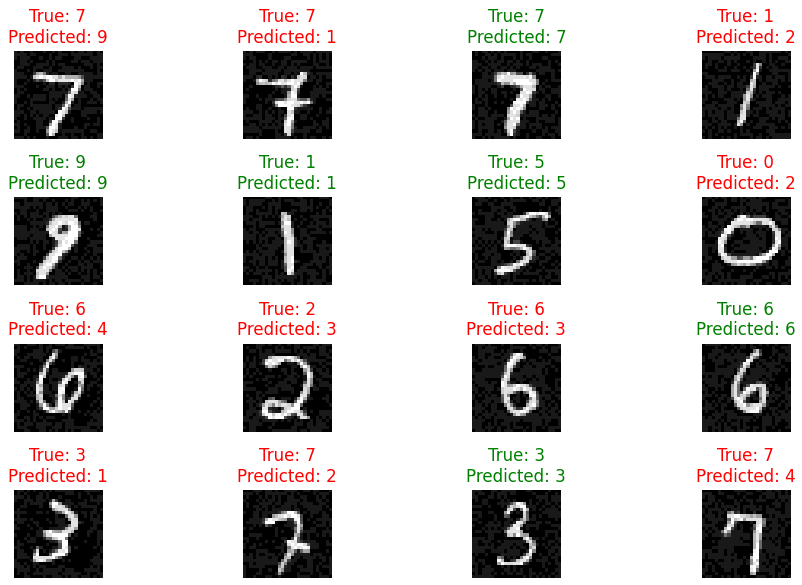
\includegraphics[width=1\textwidth]{images/fgm_attack_results.png}
    \caption{}
\end{figure}

\newpage

\subsection{Feature Adversaries}

Feature Adversaries, modelin iç özellik uzayında yanıltıcı değişiklikler yapmayı amaçlayan bir saldırı türüdür. Diğer evasion saldırıları, modelin giriş uzayında küçük pertürbasyonlar ekleyerek modelin sınıflandırma doğruluğunu bozmayı hedeflerken, Feature Adversaries, modelin ara katmanlarındaki gradyan bilgilerini kullanarak giriş verisine küçük pertürbasyonlar eklemektedir. Bu pertürbasyonlar, doğrudan ara katmandaki özellik vektörünü hedef alır ve modelin çıktısında değişiklik yapar. Bu saldırı, özellik (feature) çıkarımına dayalı derin öğrenme modellerini hedef alır ve modele olan saldırıları daha hassas hale getirmek için ara katmanları kullanarak saldırganın etkisini artırır.

\[ x_{adv} = x + \epsilon \cdot \nabla_x J(f_l(x), y) \]

Burada:

\begin{itemize}
    \item $x_{adv}$: Adversarial örnek.
    \item $x$: Orijinal giriş.
    \item $\epsilon$: Pertürbasyonun büyüklüğünü kontrol eden bir parametre.
    \item $\nabla_x J(f_l(x), y)$: Modelin $l$. katmanındaki özellik vektörüne göre girdi üzerindeki gradyanı.
    \item $f_l(x)$: Modelin $l$. ara katmanındaki özellik çıkarımı.
\end{itemize}

\subsubsection{Python Kodu}

\begin{lstlisting}[language=Python]
from art.estimators.classification import TensorFlowV2Classifier
from art.attacks.evasion import FeatureAdversariesTensorFlowV2

art_model = TensorFlowV2Classifier(
    model=model, 
    loss_object=CategoricalCrossentropy(from_logits=True), 
    nb_classes=10, input_shape=(28, 28, 1), clip_values=(0, 1))

valid_indices = np.where(
    np.argmax(y_test, axis=1)[:100] != np.argmax(y_test, axis=1)[100:200]
)[0]
source = x_test[:100][valid_indices][:32]
guide = x_test[100:200][valid_indices][:32]

feat_adv = FeatureAdversariesTensorFlowV2(
    art_model, layer=-2, delta=25/255,
    optimizer=None, step_size=1/255, max_iter=100,
)

adv_test = feat_adv.generate(source, guide)
\end{lstlisting}

\newpage

\subsection{Frame Saliency Attack}

Frame Saliency Attack, video çerçeveleri üzerinde küçük değişiklikler yaparak modelin yanlış sınıflandırma yapmasını sağlamayı amaçlar. Bu saldırı, çerçeve bazı hassasiyet haritalarını kullanarak hangi çerçevelerin modele daha fazla bilgi sağladığını tespit eder. Ardından, bu hassas çerçevelerdfe manipülasyonlar yaparak modelin davranışını bozmayı hedefler. Video içindeki her çerçeve için modelin dikkate aldığı önemli bölgeler (saliency map) hesaplanır. Bu, modelin hangi çerçeveleri veya bölgeleri daha çok dikkate aldığını gösterir. Hassas çerçeveler, modelin tahminini önemli ölçüde etkileyen çerçevelerdir. Bu çerçeveler üzerinde saldırı yapılması planlanır.

Frame Saliency Attack, bir video $V$ üzerindeki her çerçeve $F_t$ için bir saliency score $S(F_t)$ hesaplar. Modelin çıktısı $\hat{y}$:

\[ \hat{y} = f(V) \]

Burada $f$ video sınıflandırma modelidir ve $V = [F_1, F_2, ..., F_T]$ videodaki $T$ çerçeveyi temsil eder. Saliency haritası $M_t$, modein tahminine en çok katkıda bulunan çerçeveyi bulmak için kullanılır.

\[ S(F_t) = \sum_{i,j} \| \frac{\partial \hat{y}}{\partial F_t(i, j)} \| \]

Bu formülde $\frac{\partial \hat{y}}{\partial F_t(i, j)}$, çerçevenin her bir pikselinin model tahminine etkisini ifade eder. Ardından en yüksek saliency değerine sahip çerçeveler manipüle edilir.

\subsubsection{Çalışma Adımları}

\begin{enumerate}
    \item Her çerçeve için saliency map (hassasiyet haritası) hesaplanır. 
    \item Çerçevelere saliency puanı atanır ve en yüksek puanlı çerçeveler seçilir.
    \item Seçilen çerçeveler üzerinde küçük, insan tarafından fark edilemeyen değişiklikler yapılır.
    \item Manipüle edilen video modele verilir ve çıktının ne kadar değiştiği analiz edilir.
\end{enumerate}

\subsubsection{Python Kodu}

\begin{lstlisting}[language=Python]
from art.attacks.evasion import FrameSaliencyAttack, FastGradientMethod
from art.estimators.classification import TensorFlowV2Classifier

classifier = TensorFlowV2Classifier(
    model=model,
    loss_object=CategoricalCrossentropy(from_logits=True),
    nb_classes=10,
    input_shape=(32, 32, 3),
)

fgsm = FastGradientMethod(estimator=classifier, eps=0.4)
attack = FrameSaliencyAttack(classifier=classifier, attacker=fgsm)
adv_test = attack.generate(x_test[:100])
\end{lstlisting}

\begin{figure}[h]
    \centering
    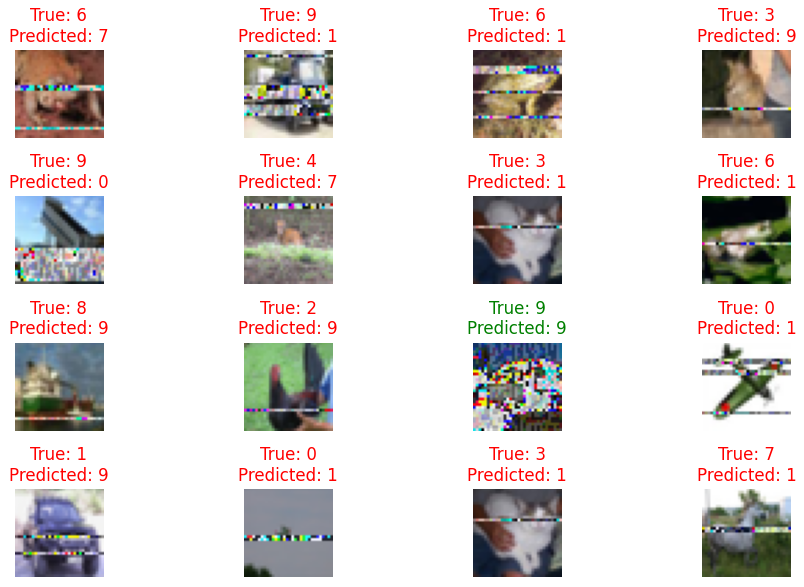
\includegraphics[width=1\textwidth]{images/frame_saliency_attack_results.png}
    \caption{}
\end{figure}

\newpage

\subsection{Geometric Decision Based Attack (G-DBA)}

Geometric Decision-Based Attack, bir modelin karar sınırlarını öğrenip bu sınırlara yakın bir noktada gürültü veya küçük değişiklikler ekleyerek modelin yanlış bir sınıflandırma yapmasını sağlar. Saldırgan, modelin nasıl çalıştığını bilmeden yalnızca verdiği tahminler üzerinden saldırıyı gerçekleştirir.

Saldırı, başlangıçta doğru sınıflandırılan $x_0$ ve yanlış sınıflandırılan $x_1$ verileriyle başlar. Amaç, $x_0$ ile $x_1$ arasında bir doğru üzerinde yer alan karar sınırına yakın $\tilde{x}$ noktasını bulmaktır. Bir saldırı noktasi $x_i$ şu şekilde tanımlanır:

\[ x_i  = (1 - \lambda) x_0 + \lambda x_1 \]

Burada $\lambda$, karar sınırına olan yakınlığı belirler. Amaç, $\lambda$'yı optimize ederek en yakın karar sınırını bulmaktır.

\[ \text{min} || f(x_i) - f(x_0) || \]

Burada $f(x)$ modelin tahmin fonksiyonudur ve saldırının amacı, $f(x_i)$'nin $f(x_0)$'dan yeterince farklı hale getirilmesidir.

\subsubsection{Çalışma Adımları}

\begin{enumerate}
    \item Hedef modelin doğru sınıflandırdığı bir giriş noktası bulunur. Ardından bu noktanın etrafında, karar sınırına en yakın yanlış sınıflandırma yapan bir giriş noktası bulunur.
    \item Modelin karar sınırına en yakın olan bu yanlış sınıflandırılmış giriş noktası kullanılarak, bir geometrik yol izlenir. Amaç, saldırının etkili olabilmesi için karar sınırının en yakınında minimum değişiklikle saldırı yapmaktır.
    \item Her iterasyonda saldırı noktası güncellenir.
\end{enumerate}

\newpage

\subsection{GRAPHITE}

GRAPHITE, graph-based techniques (graf tabanlı teknikler) kullanılarak modelin karar sınırlarını etkili bir şekilde keşfetmeyi ve bu sınırları istismar etmeyi hedefler. Saldırganlar, grafik tabanlı veri yapılarında düğümler veya kenarlar üzerinde küçük değişiklikler yaparak, modelin doğru tahmin yapmasını engelleyebilir. GRAPHITE saldırıları hem black-box (modelin iç yapısı bilinmez, sadece çıktılar üzerinden saldırı yapılır) hem de white-box (modelin iç yapısı bilinir ve model parametreleri üzerinden saldırı yapılır) senaryolarında uygulanabilir.

\subsubsection{Python Kodu}

\begin{lstlisting}[language=Python]
from art.attacks.evasion import GRAPHITEBlackbox
from art.estimators.classification import TensorFlowV2Classifier

classifier = TensorFlowV2Classifier(
    model=model,
    loss_object=CategoricalCrossentropy(from_logits=True),
    nb_classes=10, input_shape=(32, 32, 3),
    preprocessing=(0.5, 1), clip_values=(min_, max_)
)
attack = GRAPHITEBlackbox(
    classifier=classifier,  noise_size=(32, 32), 
    net_size=(32, 32),  heat_patch_size=(4, 4),
    heatmap_mode = 'Target',
)
x_adv = attack.generate(
    x=x_test[1, :, :, :][np.newaxis, :, :, :], 
    y=y_test[8][np.newaxis, :], 
    mask=None, x_tar=x_test[8,:,:,:][np.newaxis,:,:,:]
)
\end{lstlisting}

\begin{figure}[h]
    \centering
    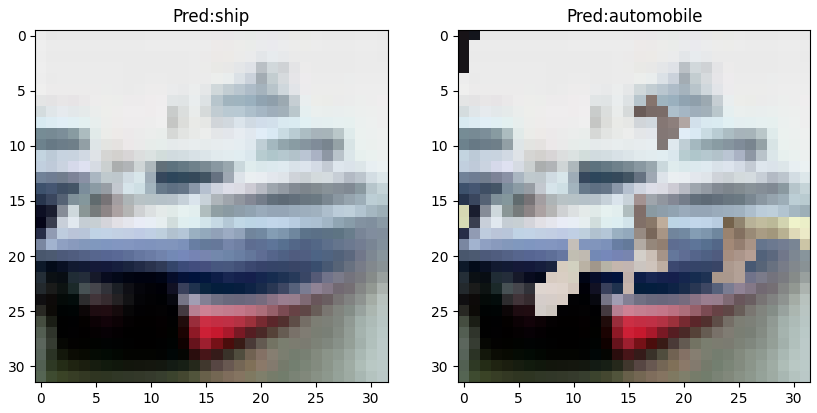
\includegraphics[width=0.6\textwidth]{images/graphite_results.png}
    \caption{}
\end{figure}

\newpage

\subsection{High Confidence Low Uncertainly (HCLU) Attack}

HCLU, bir modelin yüksek güven ile yanlış bir sınıflandırma yapmasını sağlarken, aynı zamanda modelin bu yanlış sınıflandırmada düşük belirsizlik taşımasını hedefler. HCLU saldırısı, özellikle belirsizlik ölçümlerini veya güven ölçümlerini kullanan makine öğrenimi modellerini hedef alır. Bu tür modeller, yalnızca tahminler yapmakla kalmaz, aynı zamanda tahminlerinin doğruluğuna ne kadar güvendiklerini de belirtirler. HCLU saldırısında, bir saldırgan, modelin güvenini istismar ederek, modele yanlış bir tahmin yaptırır ve model bu tahminin doğruluğuna "emin" görünür.

\newpage

\subsection{Hop Skip Jump Attack (HSJA)}

HSJA, sınırlı erişim (black-box) altında çalışan bir saldırıdır ve decision boundary keşfi ile çalışır. HSJA, modelin karar sınırlarını (decision boundary) keşfetmek için sorgulamalarda bulunarak, adversarial (yanıltıcı) örnekler üretir. Modelin sınıflandırma sonuçlarına dayanarak, girdiyi modelin karar sınırına doğru iter ve ardından bu sınırı geçip yanlış sınıflandırma yapan bir adversarial örnek üretir.

\subsubsection{Python Kodu}

\begin{lstlisting}[language=Python]
from art.attacks.evasion import HopSkipJump
from art.estimators.classification import TensorFlowV2Classifier

classifier = TensorFlowV2Classifier(
    model=model,
    loss_object=CategoricalCrossentropy(from_logits=True),
    nb_classes=10,
    input_shape=(32, 32, 3),
    preprocessing=(0.5, 1),
    clip_values=(min_, max_)
)

attack = HopSkipJump(classifier=classifier, targeted=False, max_iter=0, max_eval=1000, init_eval=10)
iter_step = 10
init_image = x_test[1]
target_image = x_test[6]
x_adv = np.array([init_image])
mask = np.random.binomial(n=1, p=0.9, size=np.prod(target_image.shape))
mask = mask.reshape(target_image.shape)

for i in range(20):
    x_adv = attack.generate(x=np.array([target_image]),
                            y=y_test[1],
                            x_adv_init=x_adv, 
                            resume=True, 
                            mask=mask)

    print(f"[Step {(i+1) * iter_step}/200] [L2 Error: {np.linalg.norm(np.reshape(x_adv[0] - target_image, [-1])):.2f}]")
    attack.max_iter = iter_step

    plt.figure()
    plt.imshow((x_adv[0] * 255).astype(np.uint))
    plt.show()
\end{lstlisting}

\newpage

\subsection{Imperceptible ASR Attack}

Imcerceptible ASR, bir ses kaydına (audio input) insan kulağının algılayamayacağı şekilde küçük ve fark edilmesi zor değişiklikler ekleyerek, ses tanıma sistemini yanıltmaktır. Imperceptible (algılanamaz) denmesinin sebebi, yapılan değişikliklerin, insanın duyusal sınırlarının ötesinde olmasıdır. Yani, orijinal ses dosyasındaki değişiklikler insanlar tarafından fark edilemez, ancak ASR sistemleri bu küçük değişiklikler yüzünden yanlış metin çıktısı üretir. Gradient tabanlı bir optimizasyon yöntemi kullanılarak, ses sinyaline küçük değişiklikler eklenir. Bu değişiklikler, insan kulağıyla fark edilmeyecek kadar küçüktür, ancak ASR sisteminin metin çıktısını değiştirebilir.

\newpage

\subsection{Basic Iterative Method (BIM)}

BIM, aynı zamanda Iterative Fast Gradient Sign Method (IFGSM) olarak da bilinir. Tek adımlı FGSM saldırısının tekrarlanmış bir versiyonudur. BIM, orijinal giriş verisine (örneğin, bir görüntüye) küçük ve tekrarlı perturbasyonlar ekleyerek modelin yanlış sınıflandırma yapmasını sağlar. Her iterasyonda, giriş verisine FGSM ile hesaplanan bir gürültü eklenir ve bu işlem, belirli bir maksimum perturbasyon seviyesine ulaşılana kadar tekrarlanır.

\subsubsection{Çalışma Adımları}

\begin{enumerate}
    \item İlk olarak, doğru şekilde sınıflandırılan bir giriş verisi seçilir.
    \item $\epsilon$, toplam pertürbasyonun maksimum büyüklüğünü belirler. $\alpha$, her iterasyonda eklenen pertürbasyonun adım büyüklüğünü belirler.
    \item Her iterasyonda, giriş verisine küçük bir pertürbasyon eklenir. Pertürbasyon, modelin kaybını maksimize edecek şekilde hesaplanır.
    \item Yeni giriş verisi $\epsilon$ sınırları içinde kliplenir, böylece pertürbasyonun toplam büyüklüğü kontrol altında tutulur.
    \item Tüm iterasyonlar tamamlandığında, son haliyle adversarial örnek elde edilir.
\end{enumerate}

\subsubsection{Python Kodu}

\begin{lstlisting}[language=Python]
from art.attacks.evasion import BasicIterativeMethod
from art.estimators.classification import TensorFlowV2Classifier

classifier = TensorFlowV2Classifier(
    model=model,
    loss_object=CategoricalCrossentropy(from_logits=True),
    nb_classes=10,
    input_shape=(32, 32, 3),
)

attack = BasicIterativeMethod(estimator=classifier, eps=0.3, eps_step=0.01, max_iter=10)
adv_test = attack.generate(x=x_test[:100])
\end{lstlisting}

\newpage

\begin{figure}[h]
    \centering
    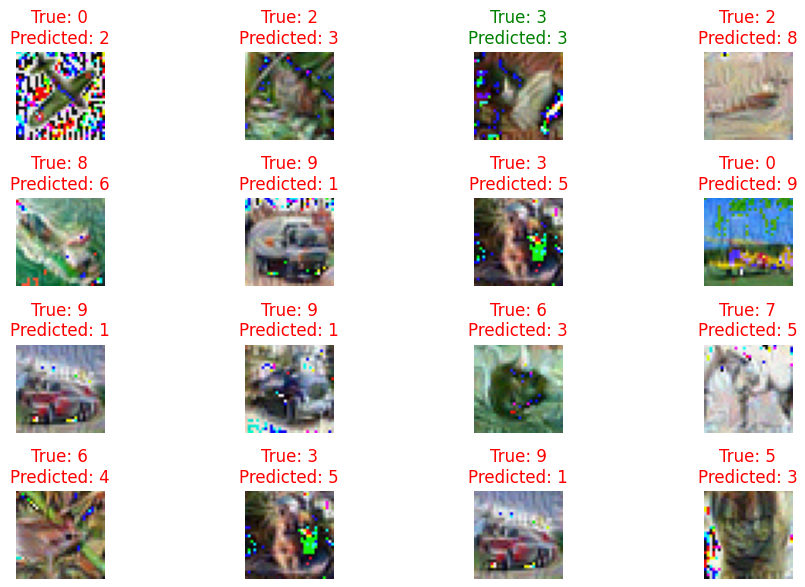
\includegraphics[width=1\textwidth]{images/basic_iterative_method_results.png}
    \caption{}
\end{figure}

\newpage

\subsection{Projected Gradient Descent (PGD)}

PGD, bir modeli hedef alan düşman örnekleri üretmek için yönlendirilmiş gradyan inişi (gradient descent) tekniğini kullanır. Amaç, modelin yanlış tahmin yapmasını sağlamak için giriş verisinin üzerine küçük ama stratejik bozulmalar eklemektir. PGD, bu bozulmaları optimize etmek için birkaç adımda küçük güncellemeler yaparak, saldırıyı daha güçlü hale getirir. PGD, aslında Basic Iterative Method (BIM) saldırısının genel bir formu olup, giriş değerlerini belirli bir norm içinde tutmak için projeksiyon kullanır.

\subsubsection{Python Kodu}

\begin{lstlisting}[language=Python]
from art.estimators.classification import SklearnClassifier
from art.attacks.evasion import ProjectedGradientDescent

art_model = SklearnClassifier(model=log_reg)
pgd = ProjectedGradientDescent(estimator=art_model, eps=0.3, 
                               eps_step=0.1, max_iter=40, targeted=False)
adv_test = pgd.generate(x_test)
\end{lstlisting}

\begin{figure}[h]
    \centering
    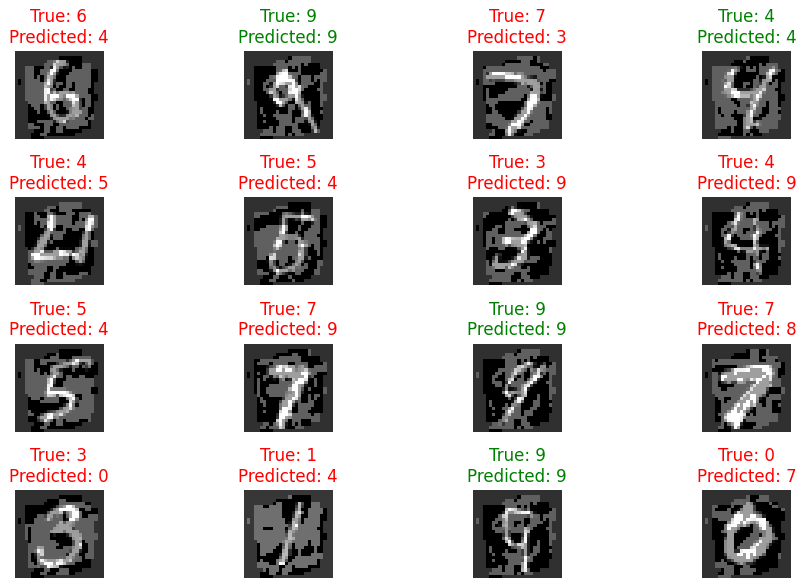
\includegraphics[width=1\textwidth]{images/pgd_attack_results.png}
    \caption{}
\end{figure}

\newpage

\subsection{Laser Attack}

Laser Attack, sensörlerin çalışma prensibini manipüle ederek işlev görür. Lazer ışınları, bir sensöre veya kameraya yönlendirilir ve bu sensörlerin topladığı verilerde gürültü oluşturur. Sensörün algıladığı lazer ışınları, gerçek dünyadaki nesnelerin algılanmasını engelleyebilir veya yanlış algılamalar yaratabilir.

\subsubsection{Python Kodu}

\begin{lstlisting}[language=Python]
from art.attacks.evasion.laser_attack.laser_attack import LaserBeamAttack

lb_attack = LaserBeamAttack(
    estimator = model,
    iterations = 50,
    max_laser_beam=(780, 3.14, 32, 32)
)

adv_images = []

for i in range(5):
    adv_image = lb_attack.generate(
        x=np.expand_dims(x_test[i], axis=0)
    )
    adv_images.append(adv_image)

adv_pred = []

for i in range(5):
    pred = model.predict(np.expand_dims(adv_images[i][0], 0))
    adv_pred.append(pred)
\end{lstlisting}

\begin{figure}[h]
    \centering
    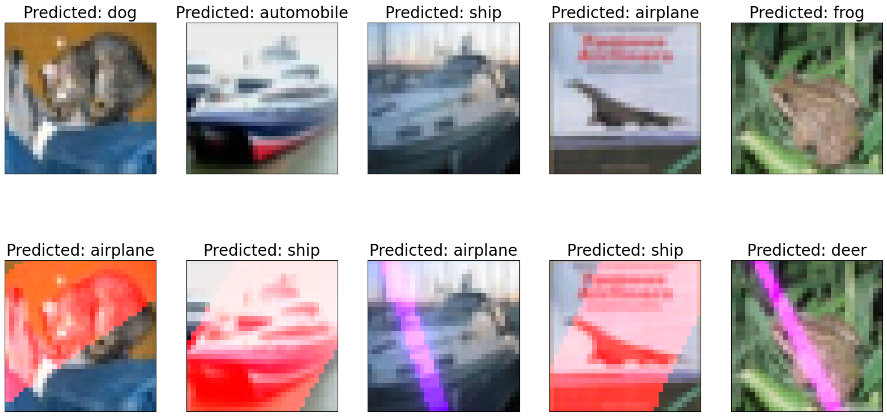
\includegraphics[width=0.6\textwidth]{images/evasion_laser_beam.png}
    \caption{}
\end{figure}

\newpage

\subsection{LowProFool Attack}

LowProFool saldırısı, girdiye uygulanan perturbasyonların düşük profilli olmasını sağlar, yani insan gözünün algılayamayacağı düzeyde minimal değişiklikler yapılır. Bu saldırının başarısı, modelin bu küçük değişikliklerle yanıltılmasında yatar.

\newpage

\subsection{NewtonFool}

Newton Fool saldırısının temel prensibi, bir girdi örneğini modelin karar sınırına iterken, Newton yönteminden yararlanarak en kısa yolu bulmaktır. Yani, modelin karar sınırına en yakın noktayı bulur ve bu noktaya ulaşacak kadar küçük perturbasyonlar ekleyerek giriş verisini adversarial bir örneğe dönüştürür.

\[ x_{k+1} = x_k - \frac{f(x_k)}{\nabla f(x_k)} \]

Burada:

\begin{itemize}
    \item $x_{k+1}$: Bir sonraki iterasyondaki girdi.
    \item $x_k$: Mevcut iterasyondaki girdi.
    \item $f(x_k)$: Sınıflandırıcı modelin çıktısı.
    \item $\nabla f(x_k)$: Sınıflandırıcı modelin çıktısına göre giriş üzerindeki gradyanı.
\end{itemize}

\subsubsection{Python Kodu}

\begin{lstlisting}[language=Python]
from art.estimators.classification import TensorFlowV2Classifier
from art.attacks.evasion import NewtonFool

art_model = TensorFlowV2Classifier(
    model=model, 
    loss_object=SparseCategoricalCrossentropy(from_logits=True), 
    nb_classes=10, input_shape=(784,), clip_values=(0, 1))
deep_fool = NewtonFool(classifier=art_model)
adv_test = deep_fool.generate(x=x_test)
\end{lstlisting}

\newpage

\subsection{Malware Gradient Descent (MGD)}

MGD, gradyan inişi algoritmasını kullanarak, bir zararlı yazılımın özelliklerini minimum değişiklikle moedlin yanlış sınıflandırmasını sağlayacak şekilde değiştirir. Amacı, girdi verisi olan zararlı yazılımı modelin karar sınırına en yakın yanlış sınıflandırma yapılacak noktaya çekmektir.

\[ x_{t+1} = x_t - \alpha \cdot \nabla J(x_t, y) \]

Burada:

\begin{itemize}
    \item $x_t$: Mevcut zararlı yazılım örneği.
    \item $\alpha$: Öğrenme oranı.
    \item $\nabla J(x_t, y)$: Zararlı yazılım örneğinin kayıp fonksiyonu J'nin gradyanı.
    \item $y$: Hedeflenen sınıf.
\end{itemize}

\newpage

\subsection{Over The Air Flickering Attack (OTA Flickering Attack)}

OTA Flickering Attack, kamera veya sensör tabanlı algılama sistemlerine yönelik görsel saldırılar yapar. Bir sahnenin veya bir nesnenin üzerine hızlı şekilde yanıp sönen (flickering) sinyaller yerleştirerek, algılama modellerini yanıltmayı hedefler. Bu sinyaller, insan gözüyle fark edilemeyen küçük değişikliklerdir, ancak kameralar tarafından algılanır ve bu sayede modelin kararlarını değiştirmek için kullanılır.

\newpage

\subsection{Pixel Attack}

Pixel Attack, hedef görüntüde sınırlı sayıda pikseli değiştirerek modelin sınıflandırma kararını değiştirmeyi amaçlar. Bu saldırı, görüntünün genel yapısını bozmadan küçük bir değişiklik yaparak saldrının fark edilmemesini sağlar.

\subsubsection{Python Kodu}

\begin{lstlisting}[language=Python]
from art.estimators.classification import TensorFlowV2Classifier
from art.attacks.evasion import PixelAttack

art_model = TensorFlowV2Classifier(model=model, nb_classes=10, 
                                   input_shape=(32, 32, 3), clip_values=(0, 1))
pixel_attack = PixelAttack(classifier=art_model, th=None, es=1)
adv_test = pixel_attack.generate(x=x_test[:16])
\end{lstlisting}

\begin{figure}[h]
    \centering
    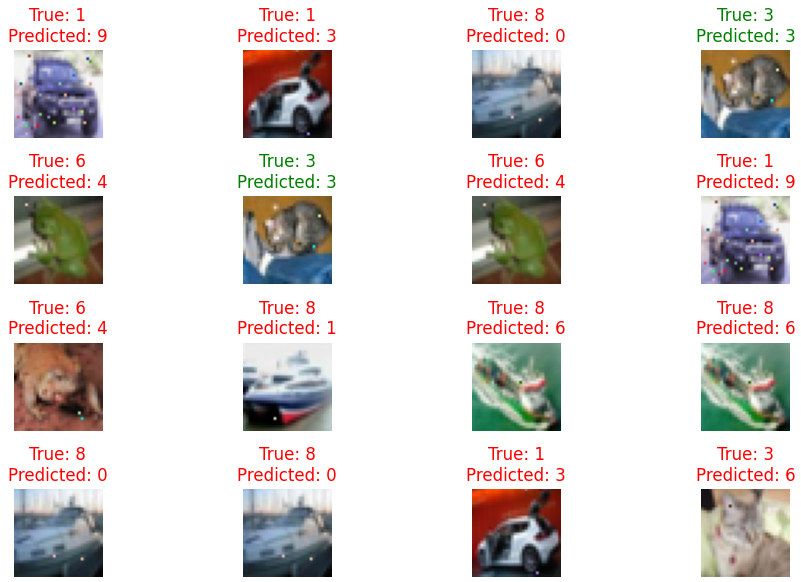
\includegraphics[width=1\textwidth]{images/pixel_attack_results.png}
    \caption{}
\end{figure}

\newpage

\subsection{Threshold Attack}

Threshold Attack, modelin çıkışının (olasılık veya karar fonksiyonu) küçük bir değişiklikle nasıl değiştiğini anlamaya çalışır. Saldırı, modelin karar sınırına yakın girdiler üzerinde uygulanarak, sınıf tahmininin değiştirilmesini sağlar.

\newpage

\subsection{Jacobian Saliency Map Attack (JSMA)} 

JSMA, modelin girdiye verdiği yanıtları analiz ederek hangi giriş özelliklerinin hedeflenen sınıfa doğru değiştirileceğini seçmek için "Jacobian Matris" kullanılarak oluşturulan bir saliency map (önem haritası) kullanır. 

\subsubsection{Python Kodu}

\begin{lstlisting}[language=Python]
from art.estimators.classification import TensorFlowV2Classifier
from art.attacks.evasion import SaliencyMapMethod

art_model = TensorFlowV2Classifier(model=model, nb_classes=10, 
                                  input_shape=(32, 32, 3), clip_values=(0, 1))
jsma = SaliencyMapMethod(classifier=art_model, theta=1, gamma=0.1)
adv_test = jsma.generate(x=x_test[:16])
\end{lstlisting}

\begin{figure}[h]
    \centering
    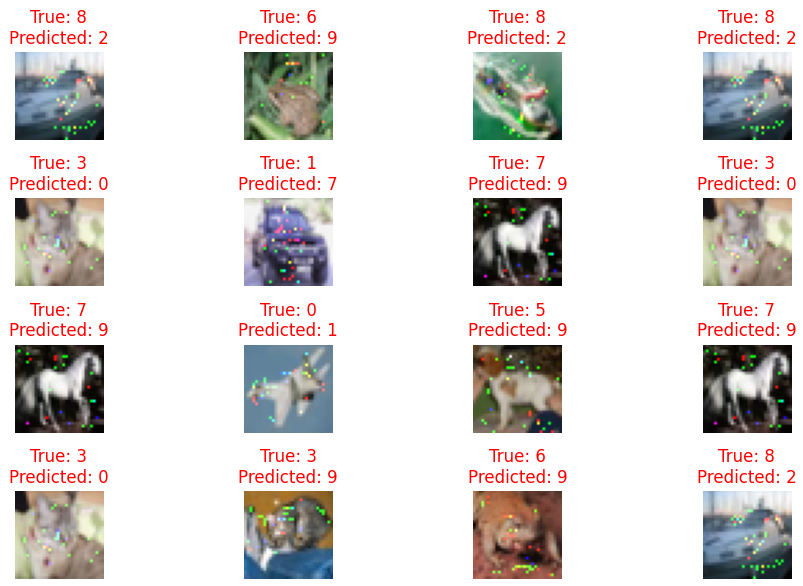
\includegraphics[width=1\textwidth]{images/jsma_results.png}
    \caption{}
\end{figure}

\newpage

\subsection{Shadow Attack}

Shadow Attack, modelin verdiği tahminlerin doğruluğunu etkilemek için girdiye küçük perturbasyonlar (bozulmalar) ekler. Bu perturbasyonlar genellikle giriş verisinde fark edilmesi zor olacak şekilde tasarlanır. Modelin çıkışlarına karşı duyarlılık analizi yaparak, hangi giriş özelliklerinin modelin kararını en çok etkilediği belirlenir ve bu özellikler hedeflenerek manipüle edilir.

\newpage

\subsection{Shape Shifter Attack}

Shape Shifter Attack, bir modelin doğru sınıflandırdığı bir görüntüyü, fark edilemeyecek kadar küçük değişikliklerle manipüle edip modelin yanlış bir sınıflandırma yapmasına neden olur.

\newpage

\subsection{Sign-OPT Attack}

Sign-OPT Attack, adversarial örneklerin optimize edilmesini sağlar. Saldırı, zeroth-order optimization yöntemini kullanarak bir hedef sınıfa ulaşmaya çalışır. Saldırının temel mantığı, modelin karar sınırlarını keşfederek küçük, insan gözüyle fark edilemeyecek değişiklikler yapmaktır. Bu değişiklikler, modelin tahmin sonuçlarını değiştirecek şekilde optimize edilir.

\subsubsection{Python Kodu}

\begin{lstlisting}[language=Python]
from art.estimators.classification import TensorFlowV2Classifier
from art.attacks.evasion import SignOPTAttack

art_model = TensorFlowV2Classifier(model=model, nb_classes=10, 
                                   input_shape=(32, 32, 3), clip_values=(0, 1))
sign_opt_attack = SignOPTAttack(estimator=art_model, targeted=False, max_iter=100, query_limit=2000)
adv_test = sign_opt_attack.generate(x=x_test[:16])
\end{lstlisting}

\newpage

\subsection{Spatial Transformations Attack}

Spatial Transformation Attack, modelin giriş verisinde uzaysal (spatial) dönüşümler yaparak modelin yanlış sınıflandırma yapmasını sağlar. Amacı, modelin hassas olduğu küçük geometrik dönüşümlerle, modelin yanlış sınıflandırma yapmasına neden olmaktır. Uzaysal dönüşümler, giriş verisinin piksel konumlarını veya yapısını değiştirir. Bu dönüşümler, küçük açısal rotasyonlar, kaydırmalar, ölçekleme veya perspektif değişimler olabilir.

\begin{itemize}
    \item \textbf{Rotation}: Görüntüde küçük açısal döndürmeler yapılır.
    \item \textbf{Translation}: Görüntüde yatay veya dikey kaydırmalar yapılır.
    \item \textbf{Scaling}: Görüntünün boyutları küçültülür veya büyültülür.
    \item \textbf{Shearing}: Görüntüye paralel kaydırmalar uygulanır.
    \item \textbf{Perspective Transform}: Görüntünün perspektifinde değişiklikler yapılır.
\end{itemize}

\subsubsection{Python Kodu}

\begin{lstlisting}[language=Python]
from art.estimators.classification import TensorFlowV2Classifier
from art.attacks.evasion import SpatialTransformation

art_model = TensorFlowV2Classifier(
    model=model, nb_classes=10, 
    input_shape=(32, 32, 3), clip_values=(0, 1)
    )
st = SpatialTransformation(
    classifier=art_model, 
    max_translation=15.0, 
    max_rotation=25.0)
adv_test = st.generate(x=x_test[:16], y=y_test[:16])
\end{lstlisting}

\newpage

\begin{figure}[h]
    \centering
    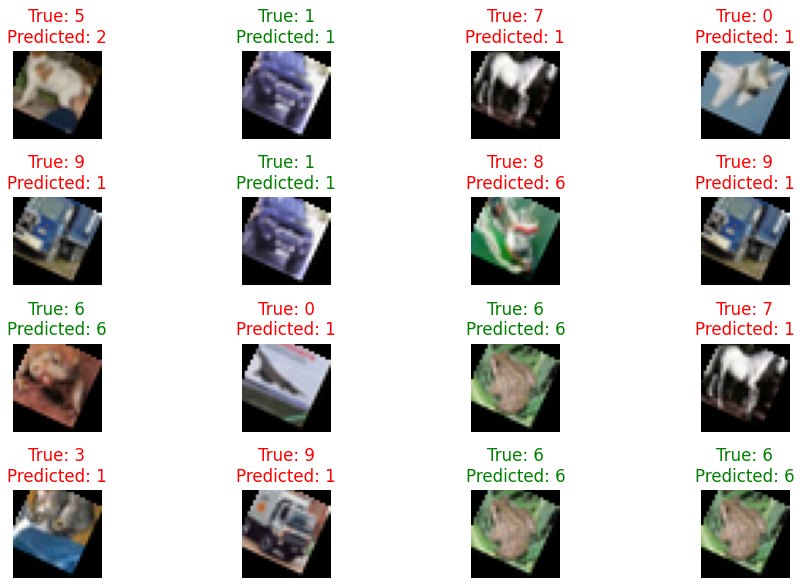
\includegraphics[width=1\textwidth]{images/spatial_transformation_results.png}
    \caption{}
\end{figure}

\newpage

\subsection{Square Attack}

Adını, giriş verisindeki belirli kare şeklindeki bölgelere yapılan manipülasyonlardan alır. Square Attack, görüntü üzerinde rastgele kare şeklinde pikselleri değiştirerek çalışır. Bu değişiklikler, modelin kararını etkileyerek yanlış sınıflandırmaya yol açabilir. Saldırı, özellikle verinin sınıflandırma sınırlarına yakın yerlerde yapılır, bu da modelin sınıflandırma doğruluğunu bozmaya yönelik etkili bir strateji sunar.

\subsubsection{Python Kodu}

\begin{lstlisting}[language=Python]
from art.estimators.classification import TensorFlowV2Classifier
from art.attacks.evasion import SquareAttack

art_model = TensorFlowV2Classifier(model=model, nb_classes=10, 
                                   input_shape=(32, 32, 3), clip_values=(0, 1))
sa = SquareAttack(estimator=art_model, norm=np.inf, max_iter=100)
adv_test = sa.generate(x=x_test[:16])
\end{lstlisting}

\begin{figure}[h]
    \centering
    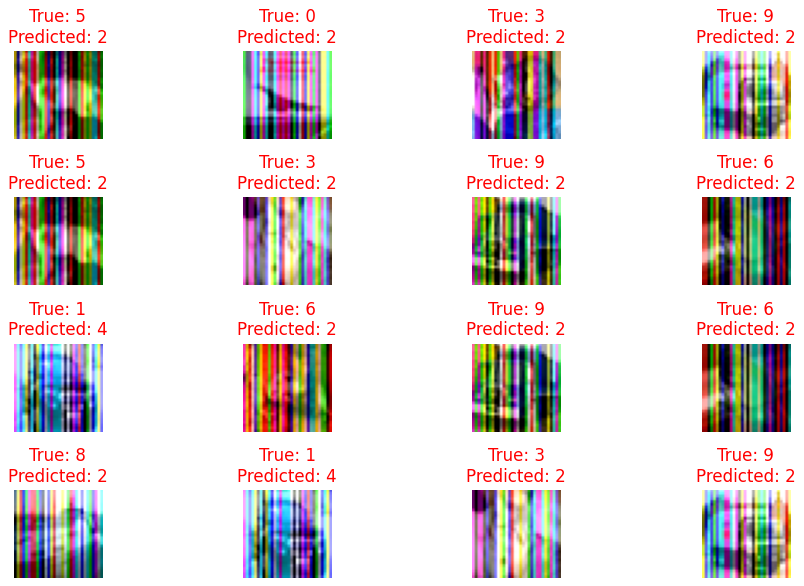
\includegraphics[width=0.8\textwidth]{images/square_attack_results.png}
    \caption{}
\end{figure}

\newpage

\subsection{Targeted Universal Perturbation Attack (T-UAP)}

T-UAP, modele evrensel bir pertürbasyon ekleyerek hedef sınıfa yönelik yanlış sınıflandırma yapılmasını sağlar. Evrensel olarak nitelendirilmesi, bir modelin üzerine eğitildiği veri setinin büyük bir kısmını etkileyebilecek tek bir pertürbasyonun bulunması anlamına gelir. Pertürbasyon, her veri noktasına eklendiğinde modelin çıkışını hedef sınıfa yönlendiren bir yapıya sahiptir.

\newpage

\subsection{Universal Perturbation Attack (UAP)}

Universal Perturbation Attack, her bir örneğe küçük bir pertürbasyon ekleyerek modelin tahminlerini yanlış yapmaya çalışır. Pertürbasyon, evrensel bir bozucu sinyal olacak şekilde optimize edilir, yani tüm veri seti üzerinde işe yarayacak şekilde ayarlanır. Model, bu pertürbasyon uygulandığında hatalı sınıflandırmalar yapar.

\newpage

\subsection{Virtual Adversarial Method (VAM)}

VAM, herhangi bir sınıflandırma etiketi kullanmadan girişlere adversarial perturbasyonlar ekler, bu yüzden "virtual (sanal)" olarak adlandırılır. VAM, denetimli olmayan adversarial örnekler oluşturarak modelin güvenliğini test eder ve sınıflandırıcının karar sınırlarını zorlar. Yarı denetimli öğrenme yöntemlerinde kullanılır.

\newpage

\subsection{Wasserstein Attack}

Wasserstein Attack, giriş verilerine minimal değişiklikler yaparak modelin tahminlerini yanıltmaya çalışır. Bu saldırı, bozucu perturbasyonların hem görünmez hem de model için anlamlı bir şekilde etkili olmasını hedefler. Bu amaçla Wasserstein mesafesi temel alınır. Amaç, giriş verilerinin orijinal dağılımından çok uzaklaşmadan modelin tahminlerini değiştiren perturbasyonlar üretmektir.

Wasserstein Attack, Wasserstein mesafesi kullanarak adversarial örnekler oluşturur. Bu mesafe, iki olasılık dağılımı arasındaki minimum taşıma maliyetini ölçer.

\[ W(p, q) = \inf_{\gamma \in \Gamma(p, q)} \mathbb{E}_{(x, y) \sim \gamma}[\| x - y \|] \]

Burada:

\begin{itemize}
    \item $p$ ve $q$: Giriş veri setinin ve bozucu pertürbasyonun olasılık dağılımları.
    \item $\Gamma(p, q)$: $p$ ve $q$ arasında ortak dağılımların kümesi.
    \item $x$ ve $y$: Girş verilerinin ve bozucu pertürbasyonların bireysel örnekleri.
    \item $\| x - y \|$ $x$ ve $y$ arasındaki mesafe.
\end{itemize}

\subsubsection{Python Kodu}

\begin{lstlisting}[language=Python]
from art.estimators.classification import TensorFlowV2Classifier
from art.attacks.evasion import Wasserstein

art_model = TensorFlowV2Classifier(
    model=model,
    loss_object=CategoricalCrossentropy(from_logits=True), 
    nb_classes=10, input_shape=(32, 32, 3), clip_values=(0, 1))
wa = Wasserstein(estimator=art_model, targeted=False, eps=0.7)
adv_test = wa.generate(x=x_test[:4])
\end{lstlisting}

\begin{figure}[h]
    \centering
    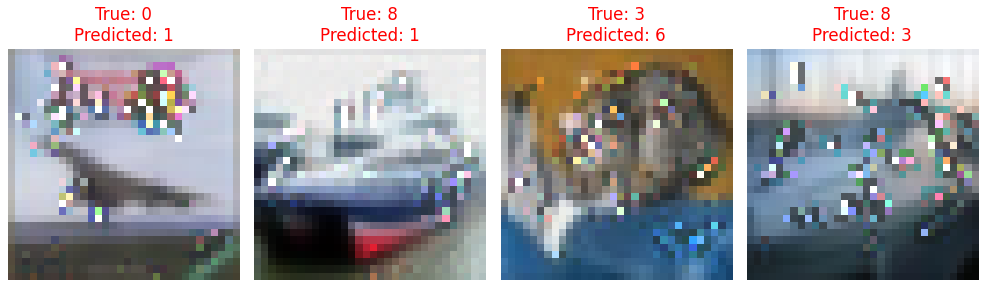
\includegraphics[width=0.7\textwidth]{images/wasserstein_attack_results.png}
    \caption{}
\end{figure}

\newpage

\subsection{Zeroth-Order Optimization (ZOO) Attack}

ZOO Attack, modelin parametrelerine veya gradyan bilgilerine ihtiyaç duymadan, doğrudan modele yapılan sorgularla saldırıyı gerçekleştirir. ZOO Attack, zeroth-order optimization (sıfırıncı derece optimizasyon) adı verilen bir yöntem kullanır. Bu yöntem, gradyan bilgisine erişmeden, sadece modelin çıktısına bakarak saldırı yapılabilmesini sağlar. Gradyanın yaklaşık bir değeri hesaplanarak optimizasyon yapılır, bu da saldırının amacına ulaşmak için yeterlidir.

ZOO Attack, gradyanı doğrudan hesaplamadığından dolayı finite-difference yöntemini kullanır. Bu yöntemde gradyan tahmini aşağıdaki gibi yapılır:

\[ \frac{\partial J(x)}{\partial x_i} \approx \frac{J(x + h e_i) - J(x - h e_i)}{2h} \]

Burada:

\begin{itemize}
    \item $J(x)$: Girdi $x$ için modelin kayıp fonksiyonu.
    \item $h$: Küçük bir adım boyutu.
    \item $e_i$: Girdi uzayındaki standart temel vektör.
    \item $\frac{\partial J(x)}{\partial x_i}$: Girdi $x$'in, $i$. bileşeni ile ilgili yaklaşık gradyan.
\end{itemize}

\subsubsection{Python Kodu}

\begin{lstlisting}[language=Python]
from art.estimators.classification import TensorFlowV2Classifier
from art.attacks.evasion import ZooAttack

art_model = TensorFlowV2Classifier(
    model=model, 
    loss_object=CategoricalCrossentropy(from_logits=True),
    nb_classes=10, input_shape=(32, 32, 3), clip_values=(0, 1))
zoo = ZooAttack(classifier=art_model, confidence=0.3, targeted=False, learning_rate=0.1)
adv_test = zoo.generate(x=x_test[:16])
\end{lstlisting}

\newpage